\documentclass[11pt]{article}
\usepackage[utf8]{inputenc}
\usepackage[english]{babel}

%Import the natbib package and sets a bibliography  and citation styles
\usepackage{natbib}
\bibliographystyle{bathx}
\usepackage{parskip} % No paragraph indents%
\setcitestyle{authoryear,open={(},close={)}} %Citation-related commands

\usepackage[a4paper,margin=2.5cm]{geometry}
\renewcommand{\familydefault}{\sfdefault} % use sans serif by default
\usepackage{graphicx}

\usepackage{url}
\usepackage{comment}
% Highlight text, \hl{}  the default colour will be yellow
\usepackage{soul}
\usepackage{xcolor}

\usepackage{hyperref} % Provides hyperlinks to sections automatically
% default formatting for links
\hypersetup{
    colorlinks=true,
    linkcolor=blue,
    filecolor=violet,      
    urlcolor=violet,
    citecolor= teal,
    pdftitle={Overleaf Example},
    pdfpagemode=FullScreen,
}

\setcounter{tocdepth}{1} % control the depth of the table (1 - Chapters and Sections, 2 - adds subsections)

\title{Agile Processes and Reflections}
\author{}

\begin{document}

\maketitle
\tableofcontents % insert the below for a table of contents
\listoffigures % it is useful to include a list of figures at least in CW2 or if you end up using a lot in CW1
\section{What is Agile?}

This is an introduction  :) 
\subsection{Mini section}
\subsubsection{An even smaller section}
\paragraph{Smaller still?}
some arbitrary text, for a picture of agile methodology see Figure~\ref{fig:agile}

% The following syntax creates a bullet point list
\begin{itemize}
\item Reason why agile great
\item Reason why agile bad
\item Reason why agile \textbf{neutral}
\end{itemize}

% An example of a numbered list, again you can do this in 'Rich Text' style
\begin{enumerate}
\item First point in numbered list
\item Second point in numbered list
\end{enumerate}

You may want to highlight some text, \hl{the default colour for this is yellow}

\includecomment{You can use this syntax as an alternative to the percentage sign for writing big blocks of comment.}
% the syntax you need in order to include graphics
% centering prevents the image from being left aligned
% Width determines how big the image is
% You can use a label so that you can reference the image within your text
% the [!h] makes the image sit within the next (experiment with removing this)
\begin{figure}[!ht]
\centering
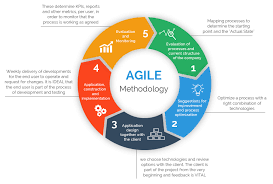
\includegraphics[width=0.7\textwidth]{agilePic}\caption{Agile methodology picture.}\label{fig:agile} 
\end{figure}

\subsection{How to cite}

Agile is great according to \citet{schwaber:2002}. To achieve this style of citation include the syntax \verb|\citet{}|



Agile is great \citep{schwaber:2002}. To include this style of citation, use \verb|\citep{}|.

An example of a citation from an online resource is \cite{WinNT}.

\section{This is my evaluation of methodology X}

%An example table
\begin{table}[htb]
\caption{An example table}
\bigskip
\begin{center}
\label{Example-Table}
\begin{tabular}{|l|l|}
\hline
Items & Values \\
\hline
\hline
Item 1 & Value 1 \\
Item 2 & Value 2 \\
\hline
\end{tabular}
\end{center}
\end{table}

\section{This is my evaluation of tool Y}
\section{This is my evaluation of practice Z}




\bibliography{thisismybib}
\end{document}


